\chapter{Ruptura espontánea de la supersimetría y el primer multiplete de \texorpdfstring{\(SU(5)\)}{SU(5)}}

\lectureoverview{La ruptura de simetría aparece aquí primero como un hecho visible en los espectros: un átomo invariante bajo rotaciones tiene niveles degenerados de momento angular, mientras que un campo magnético los desdobla. A continuación, un ferromagneto nos enseña una lección más sutil: las ecuaciones pueden conservar una simetría que el vacío no conserva. Los magnones sin brecha, la condición \(J|0\rangle\neq0\) y un parámetro de orden distinto de cero son tres descripciones de un mismo fenómeno. Trasladamos este patrón a una teoría de campos supersimétrica quiral, derivamos el potencial escalar \(V=|W'|^2\) eliminando el campo auxiliar \(F\) y distinguimos los vacíos supersimétricos de los vacíos con ruptura de \(F\). La energía del vacío resultante, el desdoblamiento entre bosones--fermiones, el goldstino, el sector oculto y el mecanismo de super-Higgs completan la discusión sobre supersimetría. La parte final cambia de tema y da paso a la gran unificación: \(SU(3)\times SU(2)\times U(1)\) se incorpora, bloque a bloque, en \(SU(5)\), cuyo primer multiplete de materia combina un doblete leptónico con tres antiquarks down.}

\section{Un espectro conserva la huella de su simetría}

El propósito de empezar con un átomo no es simplemente repasar la mecánica cuántica elemental. Los niveles de energía y las masas de las partículas son datos espectrales del mismo tipo. Si una simetría obliga a que coincidan los niveles atómicos, su ruptura puede desdoblarlos; en teoría de campos, la afirmación correspondiente es que los miembros de un multiplete de partículas pueden adquirir masas distintas.

Sea un estado atómico de momento angular total \(j\), que incluye las contribuciones del espín y del momento angular orbital. Respecto de cualquier eje elegido,
\begin{equation}
J_z|j,m\rangle=m\hbar|j,m\rangle,
\qquad
m=-j,-j+1,\ldots,j,
\end{equation}
hay \(2j+1\) estados. Las flechas habituales de los libros de texto no deben interpretarse como si el vector de momento angular solo pudiera tener \(2j+1\) direcciones espaciales posibles. Lo que está cuantizado es su componente a lo largo del eje elegido.

En el espacio vacío e invariante bajo rotaciones no hay ninguna razón física para preferir ese eje. Una rotación mezcla los estados del multiplete de espín \(j\), y la invariancia del hamiltoniano implica
\begin{equation}
[H,\mathbf J]=0,
\qquad
E_{j,-j}=E_{j,-j+1}=\cdots=E_{j,j}.
\label{eq:l9-degeneracy}
\end{equation}

\begin{classroomqa}
\audiencequestion{¿Qué simetría garantiza que rotar el átomo entero no cambie su energía? \lecturetimestamp{00:05:53}}
\lecturerresponse{La simetría rotacional. Como una rotación transforma una orientación del momento angular en otra sin cambiar el sistema físico, todos los estados \(2j+1\) tienen la misma energía.}
\end{classroomqa}

Ahora apliquemos un campo magnético \(\mathbf B=B\hat{\mathbf z}\). La interacción
\begin{equation}
H_B=-\boldsymbol{\mu}\cdot\mathbf B
\end{equation}
distingue la componente paralela al campo. Esquemáticamente,
\begin{equation}
\Delta E_m\propto mB.
\label{eq:l9-zeeman}
\end{equation}
A campo débil, los niveles con distintos valores de \(m\) se separan linealmente, y las transiciones entre ellos desdoblan las líneas espectrales.

\begin{classroomqa}
\audiencequestion{¿Cómo se llama el desdoblamiento de los niveles atómicos en un campo magnético? \lecturetimestamp{00:07:13}}
\lecturerresponse{El efecto Zeeman. Es el prototipo de toda la discusión: los niveles cuya degeneración impone una simetría se separan cuando un campo de fondo rompe esa simetría.}
\end{classroomqa}

\begin{center}
\begin{tikzpicture}[x=1.05cm,y=0.75cm,>=Latex]
  \draw[thick] (-3,0) -- (-1,0);
  \node[left] at (-3,0) {\(B=0\)};
  \foreach \y/\m in {-1.2/-1,-0.4/0,0.4/1,1.2/2} {
    \draw[thick,teal!70!black] (1,\y) -- (3,\y);
    \node[right] at (3,\y) {\(m=\m\)};
  }
  \draw[->,thick] (-0.5,0) -- (0.6,0);
  \node[above] at (0.05,0) {\(\mathbf B\neq0\)};
\end{tikzpicture}
\end{center}

\section{El ferromagneto: leyes simétricas, vacío asimétrico}

Un modelo microscópico sencillo de un ferromagneto asigna un pequeño momento magnético a cada sitio. Si los momentos vecinos reducen su energía al alinearse en paralelo, la fase de baja temperatura es ferromagnética. Si se favorece la alineación antiparalela, el resultado es antiferromagnético. En cambio, las fluctuaciones térmicas o cuánticas intensas pueden eliminar cualquier magnetización neta.

Supongamos que un ferromagneto llena el universo y se estabiliza en un estado uniformemente alineado. Su campo magnético interno desdobla los niveles de un átomo igual que lo haría un campo impuesto desde el exterior. Sin embargo, hay una diferencia decisiva. Las interacciones subyacentes no prefieren el norte, el este ni ninguna otra dirección. Todas las configuraciones rotadas uniformemente tienen la misma energía:
\begin{equation}
\mathbf M(\mathbf x)=M_0\hat{\mathbf n},
\qquad
\hat{\mathbf n}\in S^2.
\label{eq:l9-ferromagnetic-vacua}
\end{equation}
Las ecuaciones son invariantes bajo rotaciones, pero un estado fundamental concreto elige una dirección \(\hat{\mathbf n}\). Se trata de una ruptura espontánea, no explícita, de la simetría.

Un habitante formado por excitaciones de este medio no puede agarrar el universo entero y rotarlo. Por eso, localmente, la dirección elegida parece tan fundamental como un campo externo. El átomo sigue viendo el mismo patrón de niveles, con el momento angular referido a \(\hat{\mathbf n}\), en vez de a un eje \(z\) designado desde el exterior. La pregunta es cómo podría un observador interno descubrir que la asimetría aparente pertenece al estado y no a las leyes.

\subsection{El diagnóstico de Goldstone}

Una rotación uniforme de todos los momentos pasa de un vacío de la ec.~\eqref{eq:l9-ferromagnetic-vacua} a otro y no cuesta energía. Supongamos ahora que la orientación varía muy lentamente en el espacio. Los momentos vecinos ejercen entonces fuerzas unos sobre otros y la deformación se propaga como una onda de espín, cuyos cuantos son magnones. Cuando la longitud de onda tiende a infinito, la configuración se aproxima a una rotación uniforme, por lo que la energía de excitación tiende a cero:
\begin{equation}
k=\frac{2\pi}{\lambda}\longrightarrow0
\quad\Longrightarrow\quad
E(k)\longrightarrow0.
\label{eq:l9-gapless-magnon}
\end{equation}
Dos habitantes pueden hacer oscilar momentos vecinos, enviar estas ondas a través del medio y medir esta energía arbitrariamente baja. Ese experimento revela la ruptura espontánea, aunque no puedan rotar el universo.

\editorialnote{Un magnón ferromagnético no tiene brecha, pero en general presenta una relación de dispersión cuadrática no relativista \(E\propto k^2\), en vez de la relación relativista \(E\propto|k|\). En la clase se emplea el término sin masa en el sentido físicamente pertinente de brecha nula. Ambos son modos de Goldstone.}

La misma idea se aplica a las simetrías internas continuas, incluidos los grupos gauge y de sabor de la física de partículas. Sin embargo, cuando se convierte en gauge la simetría rota, el modo de Goldstone no permanece como una partícula independiente sin masa.

\begin{classroomqa}
\audiencequestion{¿Qué sucede al combinar la ruptura espontánea de simetría con la invariancia gauge? \lecturetimestamp{00:15:56}}
\lecturerresponse{El bosón de Goldstone aporta una polarización adicional al campo gauge. El bosón gauge adquiere masa: este es el mecanismo de Higgs, al que volveremos en la analogía gravitatoria.}
\end{classroomqa}

\section{Tres señales equivalentes de ruptura}

Ahora podemos describir el ferromagneto en tres lenguajes que se refuerzan mutuamente.

\paragraph{Vacíos degenerados.}
Hay un estado de energía mínima para cada orientación \(\hat{\mathbf n}\). La física tiene lugar en uno de los miembros elegidos de esta familia, aunque la simetría los relacione a todos.

\paragraph{Un generador que no anula el vacío.}
Sea \(J_a\) un generador de rotaciones. Una transformación finita es
\begin{equation}
U(\epsilon)=e^{-i\epsilon J_a},
\end{equation}
y \(J_a|0\rangle\) es proporcional al cambio infinitesimal del vacío, no al estado rotado completo.

\begin{classroomqa}
\audiencequestion{¿Cuáles son los generadores de la simetría rotacional? \lecturetimestamp{00:17:29}}
\lecturerresponse{Las componentes del momento angular total. Los llamamos \(J_a\) porque rotan todo lo que hay en el estado, no solo un átomo.}
\end{classroomqa}

Un generador no roto satisface
\begin{equation}
J_a|0\rangle=0.
\label{eq:l9-unbroken-generator}
\end{equation}
En cambio, un generador roto da
\begin{equation}
J_a|0\rangle\neq0.
\label{eq:l9-broken-generator}
\end{equation}

\begin{classroomqa}
\audiencequestion{Si \(J_a|0\rangle\) es distinto de cero, ¿simplemente devuelve el mismo vacío? \lecturetimestamp{00:19:43}}
\lecturerresponse{No. Da la diferencia infinitesimal entre el vacío elegido y otro ligeramente rotado. Físicamente, esa diferencia es una excitación de Goldstone de longitud de onda infinita.}
\end{classroomqa}

\begin{classroomqa}
\audiencequestion{¿Cambia la energía esta rotación infinitesimal? \lecturetimestamp{00:20:14}}
\lecturerresponse{No. El vacío rotado está degenerado con el original, así que el estado de Goldstone de momento nulo tiene energía cero.}
\end{classroomqa}

Simbólicamente,
\begin{equation}
J_a|0\rangle
\sim
|\pi_a,\mathbf k=0\rangle,
\label{eq:l9-generator-goldstone}
\end{equation}
donde \(\pi_a\) denota el modo de Goldstone asociado al generador roto.

\paragraph{Un parámetro de orden distinto de cero.}
La magnetización local \(\mathbf M(\mathbf x)\) es un campo. En una fase térmicamente desordenada o desordenada por fluctuaciones cuánticas,
\begin{equation}
\langle\mathbf M\rangle=0,
\end{equation}
y el vacío no selecciona ninguna dirección. En la fase ordenada,
\begin{equation}
\langle M_i\rangle\neq0
\quad\text{for at least one component }i,
\label{eq:l9-magnetization-order}
\end{equation}
de modo que una rotación mezcla esa componente distinta de cero con las demás. Los vacíos degenerados, un generador roto y un parámetro de orden distinto de cero son los tres patrones que trasladaremos a la supersimetría.

\section{Recordatorio del multiplete quiral}

El ejemplo más sencillo en cuatro dimensiones contiene un escalar complejo, un fermión de Weyl y un escalar complejo auxiliar. En coordenadas quirales,
\begin{equation}
y^\mu=x^\mu+i\bar\theta\bar\sigma^\mu\theta,
\end{equation}
un supercampo quiral puede desarrollarse esquemáticamente como
\begin{equation}
\Phi(y,\theta)=
\phi(y)+\sqrt2\,\theta\psi(y)+\theta^2F(y).
\label{eq:l9-chiral-expansion}
\end{equation}
En la clase se omite el factor convencional \(\sqrt2\); a partir de aquí lo incluimos para que los coeficientes de las componentes tengan la forma estándar. Un supercampo quiral es complejo por naturaleza: imponerle realidad no es una condición que se conserve bajo su transformación supersimétrica.

La acción cinética supersimétrica es
\begin{equation}
S_{\mathrm{kin}}
=
\int d^4x\,d^4\theta\,
\Phi^\dagger\Phi.
\label{eq:l9-kahler-action}
\end{equation}
La integración de Grassmann selecciona el coeficiente de
\(\theta^2\bar\theta^2\). Con la métrica de signatura mayoritaria negativa, el resultado en componentes es
\begin{equation}
\mathcal L_{\mathrm{kin}}
=
\partial_\mu\phi^\ast\,\partial^\mu\phi
+i\bar\psi\bar\sigma^\mu\partial_\mu\psi
+F^\ast F.
\label{eq:l9-chiral-kinetic}
\end{equation}
Los dos primeros términos describen la propagación del escalar y del fermión. El último no contiene derivadas y, por tanto, no describe ninguna partícula en propagación.

\begin{figure}[H]\centering
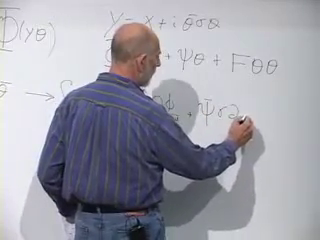
\includegraphics[width=0.76\textwidth]{lecture_09_figure_02.png}\lectureframe{00:27:36.000}\caption{La coordenada quiral y el desarrollo en componentes por encima de los términos del escalar, el fermión y el campo auxiliar.}\end{figure}

\section{Qué selecciona la integral en \texorpdfstring{\(d^2\theta\)}{d2-theta}}

Las interacciones y las masas surgen de una función holomorfa \(W(\Phi)\), el superpotencial:
\begin{equation}
S_W
=
\int d^4x
\left[
\int d^2\theta\,W(\Phi)
+\mathrm{h.c.}
\right].
\label{eq:l9-superpotential-action}
\end{equation}
Una expresión quiral no depende de forma independiente de \(\bar\theta\), de modo que integrarla respecto de las cuatro coordenadas impares daría cero. En cambio, la integral \(d^2\theta\) selecciona su componente \(\theta^2\).

Para ver la combinatoria antes de considerar una función general, sea \(W(\Phi)=\Phi^n\). En
\begin{equation}
(\phi+\sqrt2\,\theta\psi+\theta^2F)^n,
\end{equation}
hay dos maneras de obtener exactamente dos factores \(\theta\). Se puede elegir un solo \(F\theta^2\), o bien elegir dos factores fermiónicos.

\begin{classroomqa}
\audiencequestion{¿Cuántos términos contienen un \(F\theta^2\) elegido y, por lo demás, solo escalares: ¿\(n-1\) o \(n\)? \lecturetimestamp{00:31:33}}
\lecturerresponse{Hay \(n\). Cualquiera de los \(n\) factores puede aportar \(F\theta^2\); los \(n-1\) factores restantes aportan \(\phi\). La contribución es \(nF\phi^{n-1}\).}
\end{classroomqa}

\begin{classroomqa}
\audiencequestion{¿De cuántas maneras pueden dos factores aportar los dos fermiones? \lecturetimestamp{00:32:26}}
\lecturerresponse{Hay \(\binom n2=n(n-1)/2\) elecciones no ordenadas. La contracción de Grassmann fija el término \(\psi\psi\) correspondiente.}
\end{classroomqa}

Así, en la notación de la clase que omite los coeficientes,
\begin{equation}
\int d^2\theta\,\Phi^n+\mathrm{h.c.}
\;\leadsto\;
nF\phi^{n-1}
-\frac{n(n-1)}{2}\phi^{n-2}\psi\psi
+\mathrm{h.c.}
\label{eq:l9-power-extraction}
\end{equation}
El signo menos que se muestra aquí se deriva del desarrollo normalizado estándar y de la convención de Grassmann; al cambiar de convención, pueden cambiar signos aparentes.

\begin{classroomqa}
\audiencequestion{¿Qué ocurrió con el término \(\phi^n\), que no contiene ningún \(\theta\)? \lecturetimestamp{00:33:10}}
\lecturerresponse{Está presente en el producto, pero \(d^2\theta\) lo descarta. La flecha indica que la integración selecciona el coeficiente \(\theta^2\); no expresa una igualdad entre las expresiones completas.}
\end{classroomqa}

\begin{figure}[H]\centering
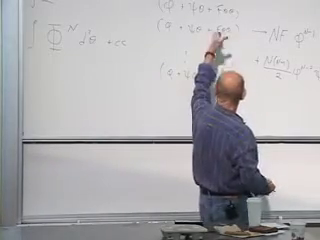
\includegraphics[width=0.82\textwidth]{lecture_09_figure_03.png}\lectureframe{00:33:38.000}\caption{Los factores de supercampo repetidos y la flecha de implicación, que extrae la componente de dos factores \(\theta\) en vez de igualarla a la expresión completa.}\end{figure}

Al sumar potencias con coeficientes arbitrarios, los factores combinatorios se convierten en derivadas:
\begin{equation}
\int d^2\theta\,W(\Phi)+\mathrm{h.c.}
\;\leadsto\;
F W'(\phi)
-\frac12 W''(\phi)\psi\psi
+\mathrm{h.c.}
\label{eq:l9-W-components}
\end{equation}

\begin{classroomqa}
\audiencequestion{¿Por qué el término fermiónico contiene \(\phi^{n-2}\), en vez de \(\phi^{n-1}\)? \lecturetimestamp{00:36:32}}
\lecturerresponse{Dos factores ya han aportado los fermiones, por lo que quedan \(n-2\) factores escalares. El coeficiente es la mitad de la segunda derivada \(W''(\phi)\).}
\end{classroomqa}

El término fermiónico es importante: da una masa cuando \(W''\) es constante y una interacción de Yukawa cuando \(W''\) depende de \(\phi\). Sin embargo, para analizar el vacío, el término auxiliar \(FW'\) proporciona la información inmediata.

\section{Eliminación del campo auxiliar}

Reunamos los términos que contienen \(F\):
\begin{equation}
\mathcal L_F
=
F^\ast F
+F W'(\phi)
+F^\ast \overline{W'(\phi)}.
\label{eq:l9-LF}
\end{equation}
Como no hay término \(\partial_\mu F\), la ecuación completa de Euler--Lagrange
\begin{equation}
\partial_\mu
\frac{\partial\mathcal L}{\partial(\partial_\mu F)}
-
\frac{\partial\mathcal L}{\partial F}
=0
\end{equation}
se reduce inmediatamente a una ecuación algebraica. Al tratar \(F\) y \(F^\ast\) como variables independientes, se obtiene
\begin{align}
\frac{\partial\mathcal L_F}{\partial F}
&=F^\ast+W'(\phi)=0,
&
\frac{\partial\mathcal L_F}{\partial F^\ast}
&=F+\overline{W'(\phi)}=0,
\label{eq:l9-F-eom}
\end{align}
y, por tanto,
\begin{equation}
F^\ast=-W'(\phi),
\qquad
F=-\overline{W'(\phi)}.
\label{eq:l9-F-solution}
\end{equation}

\begin{figure}[H]\centering
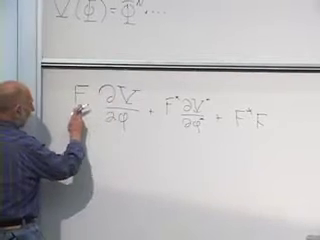
\includegraphics[width=0.82\textwidth]{lecture_09_figure_04.png}\lectureframe{00:39:40.000}\caption{La expresión completa del campo auxiliar y su ecuación de movimiento algebraica, visibles juntas tras despejar la pizarra de los elementos que las ocultaban.}\end{figure}

\begin{classroomqa}
\audiencequestion{¿No debería derivarse respecto de \(\phi\), en vez de respecto del campo conjugado que aparece escrito en la pizarra? \lecturetimestamp{00:41:21}}
\lecturerresponse{Sí. La corrección restablece el par conjugado en la ec.~\eqref{eq:l9-F-eom}: \(F^\ast=-W'(\phi)\) y \(F=-\overline{W'(\phi)}\).}
\end{classroomqa}

Al sustituir en la ec.~\eqref{eq:l9-LF} se obtiene
\begin{equation}
\mathcal L_F\big|_{\mathrm{on\ shell}}
=-|W'(\phi)|^2.
\end{equation}
Como un lagrangiano escalar tiene la forma energía cinética menos energía potencial, el potencial escalar ordinario es
\begin{equation}
\boxed{V(\phi,\phi^\ast)=|W'(\phi)|^2\ge0.}
\label{eq:l9-F-potential}
\end{equation}
Este \(V\) no es el superpotencial. Reservamos \(W\) para la función holomorfa del superspacio y \(V\) para la energía potencial ordinaria.

\subsection{Dos ejemplos inmediatos}

Con las normalizaciones convencionales exactas,
\begin{equation}
\begin{gathered}
W(\Phi)=\frac12m\Phi^2,\\
W'(\phi)=m\phi,
\qquad V=|m|^2|\phi|^2.
\end{gathered}
\label{eq:l9-quadratic-W}
\end{equation}
El mismo término da la masa del fermión
\(-\tfrac12m\psi\psi+\mathrm{h.c.}\), así que las masas del escalar y del fermión coinciden antes de que se rompa la supersimetría.

Para
\begin{equation}
W(\Phi)=\frac{g}{3}\Phi^3,
\end{equation}
se obtiene
\begin{equation}
\begin{gathered}
W'(\phi)=g\phi^2,
\qquad V=|g|^2|\phi|^4,\\
\mathcal L_{\mathrm{Yukawa}}
=-g\phi\psi\psi+\mathrm{h.c.}
\end{gathered}
\label{eq:l9-cubic-W}
\end{equation}
El vértice escalar cuártico describe la dispersión de dos escalares, mientras que el término de Yukawa es su complemento supersimétrico.

\section{Dos tipos de vacío}

El vacío es una configuración de campo constante en un mínimo de \(V\); sus términos con derivadas se anulan. Como la ec.~\eqref{eq:l9-F-potential} es no negativa, hay dos casos posibles.

\subsection{Un mínimo de energía nula}

Si existe algún \(\phi_0\) que satisfaga
\begin{equation}
W'(\phi_0)=0,
\end{equation}
entonces
\begin{equation}
V(\phi_0)=0,
\qquad
\langle F\rangle=0.
\label{eq:l9-unbroken-F}
\end{equation}
El vacío es supersimétrico. Es el análogo de la magnetización nula: ninguna componente auxiliar ha seleccionado una dirección en el superspacio.

\subsection{Un mínimo elevado}

Si las ecuaciones
\begin{equation}
W'(\phi)=0
\label{eq:l9-F-flatness}
\end{equation}
no tienen una solución simultánea en el mínimo, entonces
\begin{equation}
V_{\min}>0,
\qquad
\langle F\rangle\neq0,
\label{eq:l9-broken-F}
\end{equation}
y la supersimetría se rompe espontáneamente. La acción sigue siendo supersimétrica; su estado de menor energía, no.

\begin{figure}[H]\centering
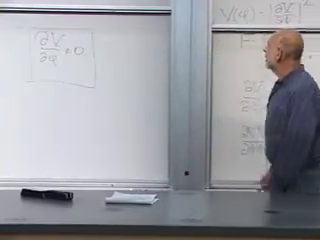
\includegraphics[width=0.88\textwidth]{lecture_09_figure_05.png}\lectureframe{00:52:09.960}\caption{La pizarra muestra el potencial positivo, la ecuación de \(F\) y la condición del vacío, y distingue las ecuaciones simétricas de una solución no simétrica.}\end{figure}

La afirmación sobre el parámetro de orden puede precisarse mediante la transformación del fermión:
\begin{equation}
\delta\psi_\alpha
=
i\sqrt2
(\sigma^\mu\bar\epsilon)_\alpha\partial_\mu\phi
+\sqrt2\,\epsilon_\alpha F.
\label{eq:l9-fermion-transformation}
\end{equation}
En un vacío homogéneo, el término con derivadas se anula. Si
\(\langle F\rangle\neq0\), la supersimetría desplaza el fermión en una cantidad constante distinta de cero, por lo que el vacío no puede ser invariante.\editorialnote{La ecuación~\eqref{eq:l9-fermion-transformation} es la forma estándar en componentes que explicita la afirmación de la clase de que las componentes del supercampo se transforman unas en otras.}

La misma conclusión se obtiene del superálgebra. En el sistema de referencia en reposo,
\begin{equation}
\{Q_\alpha,Q_{\dot\alpha}^\dagger\}
=2\sigma^0_{\alpha\dot\alpha}H.
\end{equation}
Tomar el valor esperado en el vacío expresa su energía como suma de normas de las supercargas actuando sobre él:
\begin{equation}
E_0\ge0,
\qquad
E_0=0
\ \Longleftrightarrow\
Q_\alpha|0\rangle
=Q_{\dot\alpha}^\dagger|0\rangle=0.
\label{eq:l9-algebra-vacuum-energy}
\end{equation}
Así pues, la energía positiva del vacío y la ruptura espontánea de la supersimetría son dos aspectos de una misma afirmación sobre la supersimetría global.

\begin{center}
\begin{tikzpicture}[x=1.2cm,y=1.0cm,>=Latex]
  \draw[->] (-3,0) -- (-0.2,0) node[right] {\(\phi\)};
  \draw[->] (-2.8,-0.15) -- (-2.8,2.1) node[above] {\(V\)};
  \draw[thick,teal!75!black,domain=-2.5:-0.5,samples=60]
    plot (\x,{0.65*(\x+1.5)^2});
  \fill (-1.5,0) circle (2pt);
  \node[below] at (-1.5,0) {\(F=0\)};
  \draw[->] (0.4,0) -- (3.2,0) node[right] {\(\phi\)};
  \draw[->] (0.6,-0.15) -- (0.6,2.1) node[above] {\(V\)};
  \draw[thick,orange!85!black,domain=0.9:2.9,samples=60]
    plot (\x,{0.55*(\x-1.9)^2+0.65});
  \fill (1.9,0.65) circle (2pt);
  \draw[dashed] (0.6,0.65) -- (1.9,0.65);
  \node[below] at (1.9,0.65) {\(F\neq0\)};
\end{tikzpicture}
\end{center}

\editorialnote{Una ilustración mínima es \(W=f\Phi\), para la que \(W'=f\) nunca se anula y \(V=|f|^2\). Este ejemplo de un solo campo tiene una dirección escalar plana; la ruptura estable y realista mediante términos \(F\) suele implementarse con varios campos quirales, como en los sectores ocultos de tipo O'Raifeartaigh.}

\section{Qué produce la ruptura de la supersimetría}

\subsection{Desdoblamiento de masas}

La analogía con el ferromagneto vuelve ahora a los espectros. Un campo magnético interno débil separa los niveles atómicos sin destruir la identidad del átomo. De modo similar, un parámetro de orden que rompe la supersimetría y se comunica débilmente separa los bosones y los fermiones que, de otro modo, pertenecerían a un mismo supermultiplete.

\begin{classroomqa}
\audiencequestion{¿Qué partículas se transforman unas en otras bajo la supersimetría y, por tanto, pierden la degeneración de masas cuando el vacío la rompe? \lecturetimestamp{00:51:40}}
\lecturerresponse{Los bosones y los fermiones. Sus masas ya no tienen por qué seguir siendo iguales cuando el estado deja de respetar la transformación que los relaciona.}
\end{classroomqa}

El desdoblamiento no se produce por \(\langle F\rangle\) de forma aislada; depende de los acoplamientos que transmiten la ruptura a los campos visibles. Si esos acoplamientos son débiles, las partículas visibles siguen siendo reconocibles y los desdoblamientos son pequeños en comparación con las escalas de gran unificación o de Planck. Si fueran fuertes, el análogo sería un átomo tan deformado por un campo magnético enorme que se convertiría en un objeto alargado e irreconocible.

\subsection{El goldstino}

Para un generador bosónico ordinario roto, \(J|0\rangle\) da un estado bosónico de Goldstone. Una supercarga es fermiónica y transforma estados bosónicos en fermiónicos. Como el vacío se considera bosónico, una supercarga rota crea un estado fermiónico de energía cero:
\begin{equation}
Q_\alpha|0\rangle
\sim
|\widetilde G_\alpha,\mathbf k=0\rangle.
\label{eq:l9-goldstino}
\end{equation}
Su continuación propagante es un fermión de Weyl sin masa, el fermión de Goldstone o goldstino.

\begin{classroomqa}
\audiencequestion{Si una transformación supersimétrica no deja invariante el vacío, ¿qué estado nuevo produce? \lecturetimestamp{00:53:24}}
\lecturerresponse{Un fermión sin masa. Se mantiene el patrón del teorema de Goldstone ordinario, pero un generador fermiónico transforma el vacío bosónico en el goldstino.}
\end{classroomqa}

Por tanto, la ruptura espontánea de la supersimetría global tiene dos señales inevitables:
\begin{equation}
\boxed{
V_{\min}>0
\qquad\text{and}\qquad
\text{a massless goldstino}.
}
\label{eq:l9-rigid-breaking-signatures}
\end{equation}

\section{El sector oculto}

Es útil considerar el átomo y el ferromagneto como dos sectores. El ferromagneto desarrolla el parámetro de orden; el átomo solo siente el campo que se le transmite. Cuando el acoplamiento es débil, manipular el átomo apenas excita un magnón y da poco acceso directo al medio magnético. En ese caso, el ferromagneto está oculto, aunque su presencia se infiere a partir de pequeños desdoblamientos espectrales.

La construcción de modelos supersimétricos emplea el mismo lenguaje. Campos adicionales de un sector oculto desarrollan valores esperados no nulos de términos \(F\) o \(D\). Las interacciones denominadas mecanismo de mediación comunican esa ruptura al sector visible y generan masas suaves para las supercompañeras. La transmisión débil explica cómo la teoría visible puede seguir siendo aproximadamente supersimétrica a una escala fundamental mucho más alta y, al mismo tiempo, no mostrar degeneración exacta entre bosones--fermiones a bajas energías.

La construcción no es automática. Hacen falta campos adicionales, un vacío de ruptura estable y un mecanismo de mediación controlado. Por eso, en la clase se describe la ruptura realista de la supersimetría como complicada y algo artificiosa, y no como una consecuencia única e inevitable del modelo mínimo.

\section{La gravedad modifica ambas señales}

\subsection{La energía del vacío se convierte en una fuente}

Sin gravedad, desplazar todas las energías en una constante no cambia los experimentos no gravitatorios. Con gravedad, la densidad de energía del vacío entra en la ecuación de Einstein como constante cosmológica. Un valor positivo de \(V_{\min}\) provoca una expansión acelerada. Si su escala fuera comparable a la escala de física de partículas necesaria para las masas de las supercompañeras, la curvatura resultante sería enormemente mayor que la observada.

\begin{classroomqa}
\audiencequestion{Una vez incluida la gravedad, ¿qué efecto tiene en el universo una energía del vacío positiva y distinta de cero? \lecturetimestamp{01:00:40}}
\lecturerresponse{Actúa como una constante cosmológica y provoca una expansión acelerada. A las escalas habituales de la física de partículas, el efecto sería intolerablemente grande.}
\end{classroomqa}

La supersimetría local, o supergravedad, modifica la fórmula de suma de cuadrados positivos. Para orientarnos, el potencial estándar de términos \(N=1\) \(F\) es
\begin{equation}
\begin{aligned}
V_F={}&e^{K/M_P^2}
\left(
K^{i\bar j}D_iW\,D_{\bar j}\overline W
-\frac{3|W|^2}{M_P^2}
\right),\\
D_iW={}&\partial_iW+\frac{\partial_iK}{M_P^2}W.
\end{aligned}
\label{eq:l9-sugra-potential}
\end{equation}
Debido al término negativo, en principio es posible cancelar parcialmente la energía positiva debida a la ruptura de la supersimetría. El residuo podría ser una constante cosmológica pequeña.

\editorialnote{La clase presenta intencionadamente solo una corrección esquemática y cuestiona explícitamente la ubicación de la masa de Planck. La ecuación~\eqref{eq:l9-sugra-potential} recoge la fórmula convencional para multipletes quirales con potencial de Kähler \(K\); los términos gauge \(D\) aportarían además una contribución no negativa. No explica el diminuto valor observado, que sigue siendo el problema de la constante cosmológica.}

\subsection{El mecanismo de super-Higgs}

El segundo efecto gravitatorio se entiende más fácilmente contando polarizaciones. Una partícula masiva de espín \(j\) tiene \(2j+1\) estados de espín en su sistema de referencia en reposo.

\begin{classroomqa}\audiencequestion{¿Cuántos estados de espín tiene una partícula masiva de espín \(j\)?\lecturetimestamp{01:05:16}}\lecturerresponse{\(2j+1\)En particular, una partícula masiva de espín uno tiene tres estados, mientras que un bosón gauge sin masa solo tiene helicidades \(+1\) y \(-1\).}\end{classroomqa}

La distinción es cinemática. Se puede impulsar una partícula masiva hasta el reposo y luego enviarla en una nueva dirección conservando la orientación de su espín, de modo que deben existir todas las proyecciones. No es posible adelantar a una partícula sin masa ni llevarla al reposo. Por tanto, solo puede tener las dos helicidades extremas.

Para el campo gauge electrodébil,
\begin{equation}
\underbrace{(+1,-1)}_{\text{massless vector}}
+
\underbrace{(0)}_{\text{Goldstone}}
\longrightarrow
\underbrace{(+1,0,-1)}_{\text{massive vector}}.
\label{eq:l9-higgs-count}
\end{equation}

\begin{classroomqa}
\audiencequestion{¿De dónde procede la polarización longitudinal de un \(W\) o un \(Z\) masivo? \lecturetimestamp{01:08:50}}
\lecturerresponse{Del bosón de Goldstone. El campo gauge lo absorbe, completando la representación masiva de espín uno con tres estados.}
\end{classroomqa}

La gravedad tiene un gravitón sin masa de espín dos. Su compañero supersimétrico es el gravitino sin masa de espín \(\tfrac32\).

\begin{classroomqa}
\audiencequestion{¿Cuál es el espín del gravitón y, por tanto, el de su supercompañero? \lecturetimestamp{01:10:24}}
\lecturerresponse{El gravitón tiene espín \(2\); su compañero fermiónico difiere en un medio y tiene espín \(3/2\).}
\end{classroomqa}

Un gravitino sin masa tiene helicidades \(\pm\tfrac32\), mientras que uno masivo también debe tener \(\pm\tfrac12\). El goldstino aporta precisamente esos estados que faltan:
\begin{equation}
\begin{gathered}
\underbrace{\left(+\frac32,-\frac32\right)}_{\text{massless gravitino}}
\oplus
\underbrace{\left(+\frac12,-\frac12\right)}_{\text{goldstino}}\\
\Downarrow\\
\underbrace{\left(+\frac32,+\frac12,-\frac12,-\frac32\right)}_{\text{massive gravitino}}.
\end{gathered}
\label{eq:l9-super-higgs}
\end{equation}
Este es el mecanismo de super-Higgs. Cuando la supersimetría es local, el goldstino es absorbido y deja de aparecer como una partícula independiente sin masa. El gravitino resultante interactúa gravitatoriamente y, por ello, es difícil de producir.

\section{Cambio de tema: ¿por qué \texorpdfstring{\(SU(5)\)}{SU(5)}?}

Ahora el formalismo de la supersimetría da paso a la gran unificación. El grupo gauge del modelo estándar es
\begin{equation}
G_{\mathrm{SM}}
=SU(3)_c\times SU(2)_L\times U(1)_Y.
\label{eq:l9-sm-group}
\end{equation}
Sus tres factores organizan por separado el color, el isoespín débil y la hipercarga débil. La pregunta sobre la unificación es si este producto es el subgrupo residual de un único grupo simple mayor, de modo que los multipletes de partículas y las fuerzas gauge aparentemente separados sean partes de una sola estructura. El candidato mínimo que se desarrolla aquí es \(SU(5)\).

\subsection{Elementos y generadores del grupo}

Para \(U\in SU(N)\),
\begin{equation}
U^\dagger U=\mathbf1,
\qquad
\det U=1.
\label{eq:l9-SUN-def}
\end{equation}
La primera condición expresa la unitariedad; la segunda es lo que significa ser especial. Escribamos un elemento infinitesimal como
\begin{equation}
U=\mathbf1+i\epsilon G+\mathcal O(\epsilon^2).
\label{eq:l9-infinitesimal-U}
\end{equation}
La unitariedad exige
\begin{equation}
G^\dagger=G,
\end{equation}
y
\begin{equation}
\det e^{i\epsilon G}
=e^{i\epsilon\operatorname{tr}G}=1
\end{equation}
exige
\begin{equation}
\operatorname{tr}G=0.
\end{equation}
Así pues, los generadores son matrices hermíticas sin traza.

Una matriz hermítica \(N\times N\) contiene \(N^2\) parámetros reales: \(N\) entradas diagonales reales y \(N(N-1)/2\) entradas complejas fuera de la diagonal. La condición de traza nula elimina uno. Por tanto,
\begin{equation}
\dim SU(N)=N^2-1,
\qquad
\dim SU(5)=24.
\label{eq:l9-SU5-dimension}
\end{equation}
A modo de comparación, \(SU(2)\) tiene tres generadores de Pauli y \(SU(3)\) tiene ocho generadores de color.

\section{Los bloques del modelo estándar dentro de \texorpdfstring{\(SU(5)\)}{SU(5)}}

Dividamos el espacio de cinco dimensiones en un bloque débil bidimensional y un bloque de color tridimensional:
\begin{equation}
\mathbf5=\mathbf2\oplus\mathbf3.
\end{equation}
Los generadores embebidos tienen las formas
\begin{align}
T^a_L
&=
\begin{pmatrix}
\tfrac12\tau^a&0\\
0&0_{3\times3}
\end{pmatrix},
&& a=1,2,3,
\label{eq:l9-SU2-block}\\
T^A_c
&=
\begin{pmatrix}
0_{2\times2}&0\\
0&\tfrac12\lambda^A
\end{pmatrix},
&& A=1,\ldots,8.
\label{eq:l9-SU3-block}
\end{align}
Las matrices de Pauli \(\tau^a\) generan el grupo débil \(SU(2)\); las matrices de Gell-Mann \(\lambda^A\) generan el grupo de color \(SU(3)\). Como los bloques no se superponen, los dos subgrupos conmutan.

Un generador diagonal adicional es proporcional a la identidad dentro de cada bloque y, por tanto, conmuta con ambos. En la representación fundamental, una convención conveniente para la hipercarga duplicada es
\begin{equation}
T_Y^{(\mathbf5)}=
\operatorname{diag}
\left(
1,1,-\frac23,-\frac23,-\frac23
\right).
\label{eq:l9-hypercharge-generator}
\end{equation}
Su traza se anula:
\begin{equation}
1+1-3\left(\frac23\right)=0.
\end{equation}
La representación conjugada de materia tiene los valores propios opuestos,
\begin{equation}
Y_{\overline{\mathbf5}}
=
\operatorname{diag}
\left(
-1,-1,\frac23,\frac23,\frac23
\right),
\label{eq:l9-fivebar-hypercharge}
\end{equation}
que son los valores escritos para la columna de materia en la clase. El signo global y la normalización son convencionales; estas entradas emplean la convención del modelo estándar
\begin{equation}
Q=T_3+\frac{Y}{2}.
\label{eq:l9-charge}
\end{equation}
Las ecuaciones~\eqref{eq:l9-SU2-block}--\eqref{eq:l9-hypercharge-generator} muestran
\begin{equation}
SU(3)_c\times SU(2)_L\times U(1)_Y
\subset SU(5).
\end{equation}

Los tres generadores débiles, los ocho generadores de color y el generador de hipercarga suman \(12\) de los \(24\) generadores de \(SU(5)\).\editorialnote{Los otros doce ocupan los bloques no diagonales \(2\times3\) y \(3\times2\). Sus bosones de gauge convierten componentes de tipo quark en componentes de tipo leptón, y viceversa; este es el origen estructural de las interacciones que cambian el número bariónico y leptónico, desarrolladas en la continuación.}

\begin{classroomqa}
\audiencequestion{¿Qué partículas de gauge corresponden a los generadores familiares del subgrupo? \lecturetimestamp{01:31:05}}
\lecturerresponse{Los ocho generadores de \(SU(3)\) dan lugar a los ocho gluones. Los tres generadores de \(SU(2)\) dan lugar a los campos de gauge débiles, que, tras la mezcla electrodébil, se convierten en \(W^\pm\) y en parte del sistema \(Z\)-fotón; el campo \(U(1)\) aporta la otra combinación neutra.}
\end{classroomqa}

\section{Una familia expresada en términos de campos izquierdos}

Centrémonos en la primera generación; el mismo patrón se repite para las generaciones del muón, el quark charm y el quark strange, y del tau, el quark top y el quark bottom. Lo más sencillo es contar cada campo de Weyl independiente como un campo izquierdo. Las partículas derechas se representan mediante sus campos conjugados de carga izquierdos:
\begin{equation}
Q_L=(u_L,d_L),\quad
L_L=(\nu_{eL},e_L),\quad
u^c_L,\quad d^c_L,\quad e^c_L.
\end{equation}
Sus multiplicidades son
\begin{equation}
\underbrace{6}_{Q_L}
+
\underbrace{2}_{L_L}
+
\underbrace{3}_{u^c_L}
+
\underbrace{3}_{d^c_L}
+
\underbrace{1}_{e^c_L}
=15.
\label{eq:l9-fifteen-fields}
\end{equation}

\editorialnote{El Modelo Estándar mínimo no contiene ningún campo de Weyl independiente de neutrino derecho, así que el recuento es \(15\). Este recuento, por sí solo, no afirma que el neutrino sea una partícula de Majorana. Al añadir un singlete \(\nu^c_L\), se obtienen \(16\) campos y se apunta de forma natural a \(SO(10)\), más allá de la construcción \(SU(5)\) que consideramos aquí.}

El multiplete de cinco dimensiones debe situar en las dos primeras posiciones los componentes de doblete débil sin color, y en las tres últimas, los singletes débiles con color.

\begin{classroomqa}
\audiencequestion{¿La columna propuesta contiene seis campos en vez de cinco? \lecturetimestamp{01:36:14}}
\lecturerresponse{No. Se tacha el quark up escrito en el primer intento. La columna contiene el neutrino, el electrón y tres copias de color del antiquark down: cinco componentes en total.}
\end{classroomqa}

Esto da
\begin{equation}
\overline{\mathbf5}
=
\begin{pmatrix}
\nu_{eL}\\
e_L\\
d^c_{rL}\\
d^c_{gL}\\
d^c_{bL}
\end{pmatrix}.
\label{eq:l9-fivebar}
\end{equation}
\editorialnote{La clase la denomina inicialmente, sin más, un multiplete de cinco dimensiones. En la notación estándar en la que todos los campos son izquierdos, las asignaciones de color e hipercarga la identifican como la representación conjugada \(\overline{\mathbf5}\) de \(SU(5)\).}
Los dos primeros componentes se transforman bajo \(SU(2)_L\), pero no llevan color. Los tres últimos se transforman como un antitriplete de color, pero son singletes débiles.

\begin{classroomqa}
\audiencequestion{Una vez que todos los campos se expresan como izquierdos, ¿qué quarks llevan color, pero no tienen número cuántico débil \(SU(2)_L\)? \lecturetimestamp{01:40:13}}
\lecturerresponse{Los conjugados de carga de los quarks derechos. Para este multiplete de cinco componentes, la condición de carga selecciona los tres campos de antiquark down \(d^c_{r,g,b}\).}
\end{classroomqa}

Las cargas eléctricas de la ecuación~\eqref{eq:l9-fivebar} suman cero:
\begin{equation}
0-1+\frac13+\frac13+\frac13=0.
\label{eq:l9-fivebar-charge-sum}
\end{equation}
Esto es necesario porque el operador de carga eléctrica es una combinación sin traza de generadores de \(SU(5)\).

\begin{classroomqa}
\audiencequestion{¿Por qué ocupan los tres espacios de color los antiquarks down y no los antiquarks up? \lecturetimestamp{01:43:38}}
\lecturerresponse{El neutrino y el electrón aportan una carga total de \(-1\). Los tres colores del antiquark down aportan \(+1\), con lo que la traza es cero. Tres campos de antiquark up darían una carga total incorrecta.}
\end{classroomqa}

Los diez campos izquierdos restantes son
\begin{equation}
Q_L\;(6)
\oplus
u^c_L\;(3)
\oplus
e^c_L\;(1),
\end{equation}
y encajan exactamente en la representación antisimétrica de rango dos
\begin{equation}
\mathbf{10}\cong\wedge^2\mathbf5,
\qquad
\dim\wedge^2\mathbf5=\binom52=10.
\label{eq:l9-ten-preview}
\end{equation}
La siguiente clase se ocupará de su ubicación explícita. El ajuste numérico
\begin{equation}
\overline{\mathbf5}\oplus\mathbf{10}
\end{equation}
en cada familia del Modelo Estándar constituye la primera evidencia notable de que la idea de \(SU(5)\) va más allá de un cambio de nombres arbitrario.

\begin{classroomqa}
\audiencequestion{Si el cinco y el diez son representaciones distintas, ¿significa eso que sus partículas no pueden interactuar? \lecturetimestamp{01:46:14}}
\lecturerresponse{No. Una transformación del grupo actúa dentro de cada representación irreducible, de modo que no rota directamente un elemento del cinco hasta uno del diez. Sin embargo, los dos conjuntos pueden interactuar emitiendo y absorbiendo bosones de gauge comunes, y los acoplamientos de Higgs también pueden conectar sus campos.}
\end{classroomqa}

\section{Perspectiva}

La clase ha seguido un mismo patrón a través de escalas muy distintas. La invariancia rotacional hace que los niveles atómicos sean degenerados; un campo magnético los desdobla. Un ferromagneto produce ese campo sin dejar de respetar la simetría de las leyes subyacentes, y sus magnones sin brecha revelan que la asimetría reside en el vacío. En una teoría supersimétrica quiral, el valor esperado del campo auxiliar desempeña el papel del parámetro de orden:
\begin{equation}
\begin{aligned}
\langle F\rangle=0
&\quad\Longleftrightarrow\quad
\text{unbroken supersymmetry},\\
\langle F\rangle\neq0
&\quad\Longrightarrow\quad
\text{spontaneous breaking}.
\end{aligned}
\end{equation}
En la supersimetría rígida, el vacío roto tiene energía positiva, desdobla los supermultipletes y genera un goldstino. La mediación débil motiva la introducción de un sector oculto; la gravedad convierte la energía del vacío en un problema cosmológico y absorbe el goldstino en un gravitino masivo.

La construcción de cierre con \(SU(5)\) plantea una pregunta nueva en lugar de resolverla. Los generadores hermíticos sin traza de \(5\times5\) contienen los bloques del Modelo Estándar, y los cinco primeros campos de materia encajan exactamente como \((\nu_e,e^-,d^c_r,d^c_g,d^c_b)\). Los diez restantes esperan en la representación antisimétrica. Ahí, en ese encaje aún incompleto, es donde comienza propiamente la gran unificación.
